\documentclass{report}

\usepackage[latin1]{inputenc}
\usepackage[T1]{fontenc}
\usepackage[frenchb]{babel}
\usepackage[a4paper]{geometry}
\usepackage{lmodern}
\usepackage{listings}
\usepackage{color}
\usepackage{graphicx}
\usepackage{siunitx}
\usepackage{tikz}
\usepackage{pgfplots}
\usepackage{url}
\usepackage{amsmath, amsfonts}

\pgfplotsset{compat=newest}
\usepgfplotslibrary{units}

%definition des couleurs
\definecolor{newGreen}{rgb}{0,0.6,0}
\definecolor{newOrange}{rgb}{0.87,0.39,0.15}
\definecolor{newBlue}{rgb}{0.36,0.51,0.77}
\definecolor{newMauve}{rgb}{0.58,0,0.82}

\begin{document}
\renewcommand{\chaptername}{Partie}
	\begin{titlepage}
		\vspace{-10px}
		\begin{tabular}{l}
			\textsc{Blin} S\'ebastien, \\
			\textsc{Collin} Pierre-Henri, \\
			\textsc{Louarn} Amaury 
		\end{tabular}
		\hfill \vspace{10px}
\includegraphics[scale=0.15]{ur1.png}\\
		\vfill
		\begin{center}
			\Huge{Universit\'e de Rennes 1}\\
			\large{Campus de Beaulieu}\\
			\vspace{1cm}
			\LARGE{Licence STS}\\
			\large{Cycle Pr\'eparatoire Ing\'enieur Rennes 1 - Informatique et T\'el\'ecommunications}\\
			\vspace{0.5cm}\hrule\vspace{0.5cm}
			\LARGE{\textbf{Rapport de Travail d'Initiative Personnelle Encadr\'ee (TIPE)}}\\
			\Large{Comment la reconnaissance faciale du conducteur peut-elle am\'eliorer sa s\'ecurit\'e au volant ?}
			\vfill
			\vfill
		\end{center}
		\begin{flushleft}
			\Large{Sous l'encadrement de~:}\\
			\vspace{0.2cm}
			\large{Johanne B\'ezy-Wendling}\\
			\normalsize{Ma\^itre de Conf\'erences\\
			Responsable cycle pr\'eparatoire ing\'enieur de l'Universit\'e de Rennes I\\
			(sp\'ecialit\'e informatique et t\'el\'ecommunications)}\\
			\vspace{0.2cm}
			\large{Finn J\o rgensen}\\
			\normalsize{Responsable L3 d'informatique - ISTIC}
		\end{flushleft}
		\vfill
	\end{titlepage}
	\begin{abstract}
		%TODO
	\end{abstract}
	\chapter*{Introduction}
		\subsection*{Pourquoi ce projet}
			%TODO
	\chapter{Les limites de la s\'ecurit\'e routi\`ere}
		Dans cette premi\`ere partie, nous allons aborder les limites de la s\'ecurit\'e routi\`ere, qui sont \`a l'origine de notre probl\'ematique. D'abord, nous verrons les moyens mis en oeuvre pour prot\'eger l'automobiliste. Puis, nous verrons les comportements \`a risque qui nuisent encore \`a sa s\'ecurit\'e.
		\section{Les moyens mis en place pour la s\'ecurit\'e du conducteur en France.}
			Dans le but de visualiser les moyens d\'eploy\'es par les pouvoirs publics, nous ferons dans un premier temps un historique de la s\'ecurit\'e routi\`ere depuis le d\'ebut des ann\'ees 70 (p\'eriode qui correspond \`a l'adoption des premi\`eres mesures pour diminuer le nombre de morts sur la route). Ensuite, nous verrons l'impact induit par ces moyens sur l'augmentation de la s\'ecurit\'e au volant.
			\subsection{Historique de la s\'ecurit\'e routi\`ere depuis 40 ans}

Apr\`es la seconde guerre mondiale, et en particulier d\`es le d\'ebut des ann\'ees 50, le nombre d'accidents mortels sur la route a fortement augment\'e. Plusieurs facteurs sont en cause~: l'expansion du parc automobile, un r\'eseau routier inadapt\'e, ainsi que l'insuffisante formation des conducteurs. Le premier d\'enombrement en 1954 recensa 7166 tu\'es en 3 jours. \`a cette \'epoque, la s\'ecurit\'e routi\`ere \'etait de loin un probl\`eme prioritaire pour le gouvernement car il n'y avait pas encore de politique publique.\\

\`a partir des ann\'ees 60, ce fut le d\'ebut des op\'erations de traitement des points noirs \#\#(peut-�tre des pr\'ecisions \`a apporter mais pas encore trouv\'e)\#\#. Entre 1960 entre 1970, la mortalit\'e augmenta de 55,7\% et le trafic est multipli\'e par 2,3.\\

En 1972, le Comit\'e Interminist\'eriel de la S\'ecurit\'e Routi\`ere (C.I.S.R) fut cr\'e\'e afin de d\'efinir la politique de s\'ecurit\'e routi\`ere en France. Cette ann\'ee fut aussi celle qui aura fait le plus de victimes sur les routes avec 16 545 morts. Durant la d\'ecennie qui suivie, le gouvernement instaura plusieurs mesures telles que~: les limitations de vitesse et l'obligation du port de la ceinture \`a l'avant. En dix ans, la mortalit\'e diminua de 30\% tandis que le trafic global fut multipli\'e par 1,6.\\

Au d\'ebut des ann\'ees 80, les pouvoirs publics constat\`erent une stabilisation de la baisse de la mortalit\'e routi\`ere. Ils instaur\`erent des plans d\'epartementaux de s\'ecurit\'e routi\`ere ainsi que le programme R.E.A.G.I.R (R\'eagir pour les Enqu�tes sur les Accidents Graves et les Initiatives pour y Rem\'edier). Ce fut \'egalement le d\'ebut de la politique locale de s\'ecurit\'e routi\`ere. Entre 1980 et 1990, le seuil d'alcool\'emie autoris\'e fut abaiss\'e de 1,2 \`a 0,8 g/l d'alcool dans le sang, la plupart des v\'ehicules furent \'equip\'es d'un syst\`eme anti-blocage des roues, le nombre de carrefours giratoires augmenta (diminution notable du nombre d'accidents mortels dans les carrefours).\\

\`a la fin des ann\'ees 80, un livre blanc de la s\'ecurit\'e routi\`ere fut publi\'e dans le but d'\'enoncer les orientations majeures des futures politiques de s\'ecurit\'e routi\`ere. Entre 1990 et 2000, de nombreuses mesures furent donc mises en oeuvre~: en 1990, la vitesse maximale autoris\'ee en agglom\'eration fut fix\'ee \`a 50km/h et un permis \`a points fut instaur\'e, le taux d'alcool autoris\'e dans le sang se limita \`a 0,5 g/l, l'essentiel du r\'eseau autoroutier \'etait quasiment achev\'e, la plupart des v\'ehicules furent \'equip\'es d'airbags. De plus, le continuum \'educatif est mis en place. D'apr\`es le site gouvernemental de la s\'ecurit\'e routi\`ere, le continuum \'educatif exprima l'id\'ee que "l'\'education \`a la s\'ecurit\'e routi\`ere ne se fait pas seulement lors du passage du permis de conduire, mais tout au long de sa vie".\\
En dix ans, le trafic global augmenta de 20\%, alors que la mortalit\'e routi\`ere diminua d'autant.\\

En 2002, la s\'ecurit\'e routi\`ere \'etait l'un des principaux chantiers du Pr\'esident de la R\'epublique. Un an plus tard, les premiers radars de contr�le/sanction automatiques //--syst\`emes de sanction automatique--// arriv\`erent au bord des routes. La m�me ann\'ee, le Conseil National de la S\'ecurit\'e Routi\`ere (C.N.S.R) s'installa \#\#pr\'eciser ses missions\#\#. En 2004, le permis probatoire fit son apparition. Les sanctions sont devenues plus importantes pour les conducteurs en \'etat d'\'ebri\'et\'e. En effet, un d\'epassement du taux l\'egal d'alcool dans le sang entraine un retrait de six points sur le permis de conduire. En 2000 et 2010, la mortalit\'e baissa de 51,1\% alors que le trafic global augmenta de 7\%.\\

Apr\`es un bref aper�u sur l'\'etendu des d\'ecisions prises par les gouvernements depuis 1972 en mati\`ere de s\'ecurit\'e routi\`ere, nous allons maintenant voir quel est le bilan de ces mesures.\\

\subsection{Bilan de quarante ann\'ees de mesures}

Premi\`erement, le nombre de tu\'es sur la route a fortement diminu\'e depuis 1972 (ann\'ee qui marque la fin de la hausse constante de la mortalit\'e routi\`ere). Comme nous pouvons le constater sur le graphique ci-dessus/ci-dessous, ce nombre a \'et\'e divis\'e par plus de quatre en quarante ans malgr\'e un doublement du parc automobile. En 2012, 3 653 personnes ont \'et\'e tu\'ees en 30 jours contre plus de 18 000 en 1972.\\

%Image[\'evolutionscompar\'eetraficetmortalit\'erouti\`ereann\'ees1948\`a2011.png]

Ces progr\`es observ\'es en mati\`ere de s\'ecurit\'e routi\`ere ont \'et\'e obtenus en agissant sur plusieurs facteurs. Lors d'un accident, quatre facteurs essentiels doivent �tre pris en compte~: tout d'abord les facteurs li\'es \`a l'infrastructure (conception, entretien et exploitation), les facteurs li\'es aux v\'ehicules (s\'ecurit\'e passive et active), les facteurs li\'es aux comportements des usagers (formation, communication, r\'epression), et le progr\`es des services de secours et de soin. Cependant, il est tr\`es difficile de d\'efinir la part de chacun de ces facteurs dans l'am\'elioration de la s\'ecurit\'e routi\`ere. \\

Concernant les facteurs li\'es \`a l'infrastructure, nous pouvons retenir plusieurs points qui ont particip\'e \`a l'am\'elioration de la s\'ecurit\'e routi\`ere~: comme la construction d'un r\'eseau autoroutier, le d\'eploiement de barri\`eres de s\'ecurit\'e le long des routes potentiellement dangereuses, les protections anti-\'eblouissements, des bandes sonores anti-endormissement, les bandes d'arr�ts d'urgences. \\

Ensuite parmi les facteurs li\'es aux v\'ehicules, la situation actuelle n'a plus rien \`a voir avec celle d'il y a quarante ans. Le port obligatoire de la ceinture, l'obligation pour les enfants de s'asseoir \`a l'arri\`ere du v\'ehicule, l'apparition de diff\'erents coussins gonflables de s\'ecurit\'e dans le poste conducteur (airbags), la structure des v\'ehicules qui absorbent mieux les chocs (\`a l'aide des pare-chocs par exemple) ont eu un impact consid\'erable sur la diminution de la gravit\'e des accidents. Nous pouvons aussi \'evoquer la mise en place progressive dans tous les v\'ehicules de syst\`emes d'aide \`a la conduite (ABS par exemple). \\

Les facteurs li\'es aux comportements des usagers sont s�rement ceux qui ont eu le plus d'effets sur la diminution du nombre de tu\'es sur la route. Tout d'abord, la formation des usagers qui n'a cess\'e de cro\^itre au fil des ann\'ees a permis de leur donner une meilleure appr\'ehension de la route. Cette formation s'inscrit dans un processus progressif et continu. Que ce soit en famille, \`a l'\'ecole, lors du passage du permis de conduire, ou pendant le reste de leur vie. Ensuite, la r\'epression a incit\'e les usagers \`a respecter les nouvelles mesures de s\'ecurit\'e mises en place. Par exemple, sur le respect des limitations de vitesse, du taux d'alcool\'emie pr\'esent dans le sang, du port de la ceinture, etc. Au fil du temps, la r\'epression s'est durcie avec l'augmentation des points retir\'es en cas de d\'elit. Enfin, la communication sur la s\'ecurit\'e routi\`ere a \'et\'e primordiale pour faire changer les moeurs.
Des campagnes publicitaires (voir ci-dessous) parfois chocs ont fait prendre conscience aux usagers que nous sommes "tous responsables" (slogan utilis\'e lors des campagnes de pr\'evention).\\

%Image[karl-for-Securit\'e-Routiere.jpg]
 
Suite \`a cette pr\'esentation des moyens mis en oeuvre par les gouvernements successifs et de leurs impacts sur la s\'ecurit\'e routi\`ere, nous allons \`a pr\'esent aborder les limites de ces mesures, c'est-\`a-dire les comportements qui mettent en p\'eril cette s\'ecurit\'e.\\

\section{Les comportements \`a risques}

Malgr\'e toutes les mesures prises pour prot\'eger le conducteur, de nombreux accidents mortels ont encore lieu. La plupart du temps, cet accident n'est pas d� \`a une d\'efaillance du v\'ehicule, une route endommag\'ee ou encore au mauvais temps, mais \`a une d\'efaillance humaine. C'est pourquoi, nous analyserons d'abord les principales causes des accidents, puis un type de comportement dangereux en particulier~: la conduite \`a l'aveugle.

\subsection{Les principales causes d'accidents}

Les accidents corporels sont g\'en\'eralement d\'etermin\'es par plusieurs facteurs.Ces facteurs peuvent influer sur l'occurrence des accidents, mais aussi sur leur gravit\'e. Ils sont souvent li\'es entre eux, et il est particuli\`erement difficile de d\'eterminer le facteur principal, habituellement appel\'e la "cause" de l'accident.\\

La vitesse est un facteur pr\'epond\'erant dans les accidents corporels. C'est \'egalement un facteur transversal, car la vitesse est presque toujours pr\'esente comme facteur d'occurrence et/ou facteur de gravit\'e. En 2011, en France, au moins 26\% des accidents mortels ont pour cause identifi\'ee la vitesse d'apr\`es les forces de l'ordre. En Suisse et en Allemagne la vitesse, seule ou associ\'ee, repr\'esente 40\% des accidents mortels.\\

L 'alcool est \'egalement un facteur majeur pr\'esent dans les accidents. En effet, s'il est pr\'esent dans le sang en quantit\'e trop importante, il entra\^ine une augmentation de la vitesse, la somnolence, l'oubli du port de la ceinture de s\'ecurit\'e. Le taux d'implication de l'alcool dans la mortalit\'e routi\`ere reste constant~: environ 31\%.Les 875 accidents mortels avec au moins un conducteur ayant une alcool\'emie sup\'erieur au seuil autoris\'e ont provoqu\'e 964 victimes. Parmi les victimes des accidents mortels avec comme facteur l'alcool, les conducteurs ainsi que leurs passagers repr\'esentent 70\% des personnes tu\'ees.\\

Les autres facteurs sont~:
\begin{itemize}
	\item{L'usage des stup\'efiants (en 2011, 455 accidents mortels avec au moins un conducteur test\'e positivement aux stup\'efiants). Ces accidents ont entrain\'es le d\'ec\`es de 499 personnes (soit 13\% de la mortalit\'e routi\`ere).}
	\item{La prise de m\'edicaments~: une \'etude r\'ealis\'ee par une \'equipe de l'INSERM (projet CESIR-A) a montr\'e que 3\% des accidents \'etaient attribuables \`a la prise de produits m\'edicamenteux.}
	\item{le respect des distances de s\'ecurit\'e. D'apr\`es le Code de la Route~: \og Lorsque deux v\'ehicules se suivent, le conducteur du second doit maintenir une distance de s\'ecurit\'e suffisante pour pouvoir \'eviter une collision en cas de ralentissement brusque ou d'arr�t subit du v\'ehicule qui le pr\'ec\`ede. Cette distance est d'autant plus grande que la vitesse est plus \'elev\'ee. Elle correspond \`a la distance parcourue par le v\'ehicule pendant un d\'elai d'au moins deux secondes\fg. Globalement, plus de 50\% des conducteurs ne respectent pas cette r\`egle. Or, le non-respect des distances de s\'ecurit\'e qui entrainent des collisions par l'arri\`ere et des collisions en chaine totalise 6.2\% de la mortalit\'e routi\`ere.}
	\item{Le port de la ceinture~: en 2011, 22\% des personnes tu\'ees n'\'etaient pas ceintur\'ees.}\\
\end{itemize}

Comme nous venons de le voir, les principales causes d'accidents mettent en avant le comportement de l'usager. Nous allons nous attarder sur une une cause d'accident qui n'a pas \'et\'e \'evoqu\'ee pr\'ec\'edemment~: la distraction du conducteur.\\

\subsection{La conduite \`a l'aveugle}

La conduite \`a l'aveugle fait r\'ef\'erence au rel�chement d'attention du conducteur pour effectuer d'autres t�ches annexes \`a l'int\'erieur du v\'ehicule. Ainsi, ses capacit\'es d'analyse de la circulation et de r\'eaction sont fortement diminu\'ees.\\

Il existe trois types de distraction~: visuelle (regarder autre chose que la route), manuelle (d\'etacher ses mains du volant), cognitive (ne pas �tre concentr\'e sur la route). Concr\`etement, cela signifie~: utiliser sont t\'el\'ephone portable ou un smartphone, envoyer un sms, manger et boire, parler aux passagers, se maquiller, lire (y compris les cartes), utiliser un syst\`eme de navigation, regarder une vid\'eo, r\'egler la radio, un lecteur CD ou mp3, etc. Envoyer des sms est la distraction la plus dangereuse, car elle combine les trois types de distraction. De plus, envoyer ou lire un texte oblige \`a quitter des yeux la route pendant 4,6 s en moyenne. A 55 mph (environ 88 km/s), c'est comme conduire la longueur d'un terrain de football, les yeux band\'es.\\

En France, certaines \'etudes ont montr\'e que 25\% \`a 50\% des accidents corporels \'etaient dus \`a la distraction du conducteur. A l'\'etranger, la conduite \`a l'aveugle est \'egalement un facteur de plus en plus important dans la mortalit\'e routi\`ere. Par exemple, chaque jour aux Etats-Unis, plus de 9 personnes sont tu\'ees et plus de 1,060 personnes sont bless\'ees dans des accidents o\`u sont impliqu\'es un conducteur distrait. Par ailleurs, beaucoup d'usagers (en particuliers les jeunes) ne semblent pas encore avoir pris conscience du danger de ces pratiques. En effet, d'apr\`es un sondage r\'ealis\'e en 2011 aux Etats-Unis, 69\% des conducteurs �g\'es de 18 \`a 64 ans avaient t\'el\'ephon\'e en conduisant (En Europe, ce taux varie entre 21\% au Royaume-Uni \`a 59\% au Portugal) et 31\% avaient lu ou envoy\'es un sms en conduisant dans les 30 derniers jours avant d'�tre sond\'es.\\

	\chapter{La reconnaissance faciale}
		Dans cette deuxieme partie, nous nous pencherons sur la reconnaissance faciale. Dans un premier temps, nous \'etudierons l'aspect th\'eorique de la reconnaissance, puis  l'aspect exp\'erimental.

\section{Th\'eorie}

Afin d'\'etudier l'aspect th\'eorique de la reconnaissance faciale, nous allons d'abord l'aborder de fa�on g\'en\'eral. Ensuite, nous analyserons plus en d\'etail diff\'erentes m\'ethodes de reconnaissance~: Eighenface, Fisherface et LBPH.

\subsection{G\'en\'eralit\'es}

Apr\`es des recherches approfondies, nous avons pu constater qu'il existe \'enorm\'ement de m\'ethodes possibles pour reconna�tre un visage.  Ces m\'ethodes peuvent \'egalement �tre combin\'ees entre elles (par exemple, la mise en place en place d'un r\'eseau neuronal \#\#explication peut-�tre ?\#\#). Cependant, en trois mois, nous nous n'aurions pas eu le temps de mettre en place une telle m\'ethode.\\

Par ailleurs, nous avons choisi de traiter uniquement des images en noir et blanc, car la colorim\'etrie a tr\`es peu d'impact dans le processus de reconnaissance.\\

\subsection{La m\'ethode Eighenface}

La m\'ethode de reconnaissance faciale Eighenface a pour particularit\'e de se baser sur des \og eighen vectors\fg, c'est-\`a-dire des vecteurs propres.\\

L'algorithme est le suivant~: chaque image est consid\'er\'ee comme un vecteur avec pour dimension son nombre de pixels. Puis, un ou plusieurs algorithmes recherchent les principales composantes //--plus de pr\'ecision sur composante ?--//. A l'aide de plusieurs images du m�me visage, nous pouvons alors composer une image du visage \og moyen\fg qui contiendra \'egalement les principales composantes (l'eighenface). La m\'ethode de reconnaissance des axes principaux est d\'etaill\'ee ici~: Matthew Turk and Alex Pentland. Eigenfaces for recognition. J. Cognitive Neuroscience. 3(1)~:71{86, 1991}. Enfin, il suffit de comparer l'eighenface et les composantes principales d'une capture d'un visage.\\

L'avantage de cette m\'ethode est la connaissance de son existence depuis longtemps. Cependant, elle pr\'esente \'egalement des d\'esavantages non-n\'egligeables. En effet, comme chaque pixel est une dimension, une image $100\times100$ donne 10000 vecteurs \`a traiter. Le nombre de donn\'ees \`a analyser est donc trop important.\\

\subsection{La m\'ethode Fisherface}

La m\'ethode de reconnaissance faciale Fisherface se base sur les travaux de Sir R.A. Fisher. L'id\'ee de base de l'algorithme est la suivante~: toutes les images qui se ressemblent, se retrouvent proches. Concr\`etement, imaginons un espace d'images comprenant une \'echelle repr\'esentant les visages. Si nous projetons les images sur l'\'echelle, nous pouvons dire que //-- je n'ai pas compris la suite --//\\

\begin{figure}[h]
	\begin{center}
		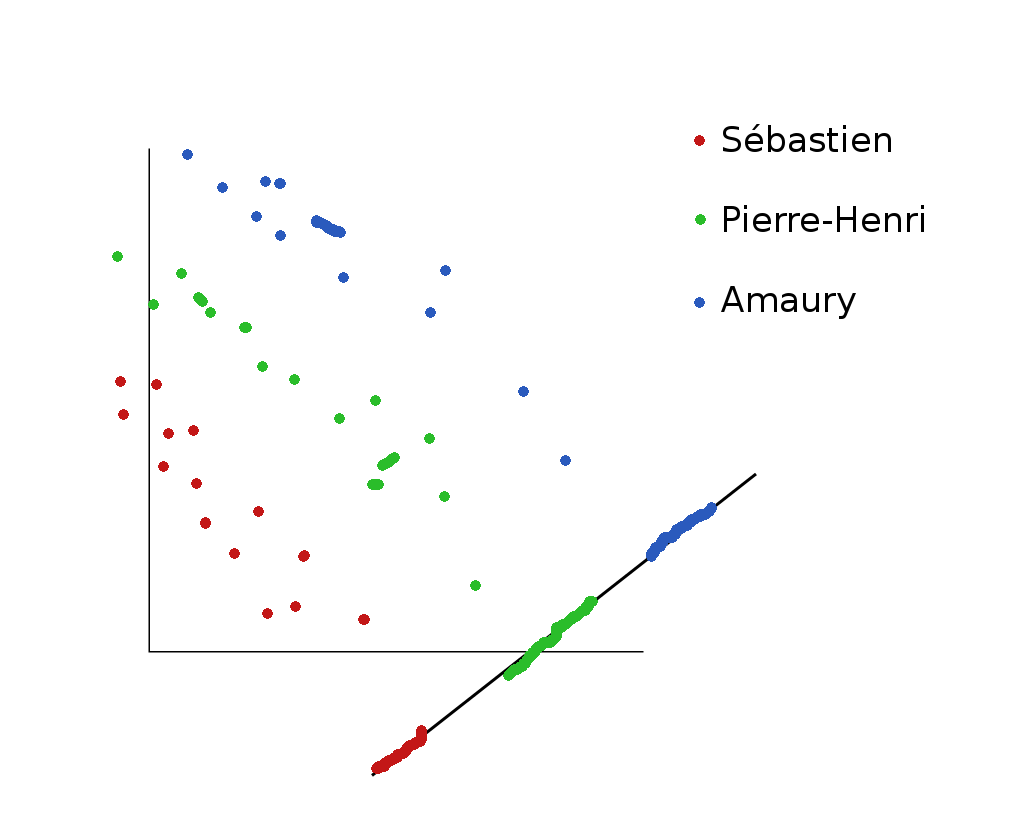
\includegraphics[scale=0.3]{images/fisherfacedistrib.png}
		\caption{Distribution Fisherface}
	\end{center}
\end{figure}

Pour plus de d\'etails~: \url{http://docs.opencv.org/modules/contrib/doc/facerec/facerec_tutorial.html#fisherfaces}.\\

Globalement, cette m\'ethode pr\'esente les m�mes avantages et inconv\'enients que la m\'ethode Eighenface. Cependant, elle est moins sensible \`a la lumi\`ere et \`a la d\'eformation des visages car elle ne se base pas sur des composantes discriminatoires.\\

\subsection{La m\'ethode LBPH}

La m\'ethode de reconnaissance faciale LBPH (Local Binary Patterns Histogram) consiste \`a visualiser la valeur d'un pixel (moyenne des trois composantes RGB) par rapport aux pixels voisins.\\

Pour commencer, l'image est divis\'e en groupe de pixels. Chaque groupe de pixels correspond \`a une matrice carr\'e contenant les valeurs des pixels. Puis, le pixel plac\'e au centre de la matrice est choisi comme valeur de r\'ef\'erence. Ensuite, toutes les valeurs de la matrice sont remplac\'ees soit par 0, soit par 1 en fonction de leur valeur. La fonction d'Heaviside, nous dit que 
\[
	\forall x \in \mathbb{R}, H(x)=
	\left \{
	\begin{array}{l l}
		0 & \text{si } x \leq 0\\
		1 & \text{sinon}
	\end{array}
	\right.
\]
Ici, si nous attribuons la valeur 0 si la valeur du pixel est inf\'erieur \`a la valeur du pixel de r\'ef\'erence, 1 sinon. Apr\`es cette op\'eration, chaque pixel du groupe est pond\'er\'e avec un poids plus ou moins fort (le pixel en haut \`a gauche a le poids le plus faible, tandis que le pixel en bas \`a droite a le poids le plus fort). Ainsi, nous obtenons un nombre binaire qui donne une certaine valeur en base 10. Tous les groupes de l'image sont soumis \`a ce processus pour finalement obtenir un histogramme de l'image. Enfin, il ne reste plus qu'\`a faire la diff\'erence entre deux histogrammes pour comparer deux images.\\

Cet algorithme est tr\`es utilis\'e comme nous pouvons le voir dans~: Facial expression recognition based on Local Binary Patterns:A comprehensive study de Caifeng Shan a, * , Shaogang Gong b , Peter W. McOwan b, o\`u il est combin\'e avec Adaboost (plugin d'openCV) pour obtenir de meilleurs r\'esultats, et un r\'eseau neuronnal. Mais aussi dans~: Face Recognition with Local Binary Patterns, Spatial Pyramid Histograms and Naive Bayes Nearest Neighbor (NBNN) classification de Daniel Maturana, Domingo Mery and Alvaro Soto o\`u les auteurs essayent d'am\'eliorer l'algorithme dans le but d'en cr\'eer un nouveau~: NBNN. Nous n'utiliserons pas cet algorithme par manque de temps, mais \'egalement car LBPH est d\'ej\`a pr\'esent dans openCV.\\

Comme nous venons de le voir, il existe diff\'erents m\'ethodes 

		\section{Exp\'erimentations}
			\subsection{Protocole}
				%TODO
			\subsection{R\'ealisation}
				%TODO
			\subsection{R\'esultats et analyse}
				%TODO
				%GRAPHIQUES A DEPLACER~:
				\begin{figure}
					\begin{center}
					\begin{tikzpicture}
						\begin{axis}[
							width=12cm,
							height=7cm,
							xlabel={nombre d'images dans la base de donn\'ee},
							ylabel={temps d'ajout},
							y unit=\si{\second},
							legend style={at={(0.23,0.95)},anchor=north},
							legend entries={eigenface,fisher face,LBPH}
						]
							\addplot  table[x=nb,y=tps,col sep=comma] {data/ByNumberOfImages_rec_eigenface.csv};
							\addplot  table[x=nb,y=tps,col sep=comma] {data/ByNumberOfImages_rec_fisherface.csv};
							\addplot  table[x=nb,y=tps,col sep=comma] {data/ByNumberOfImages_rec_LBPH.csv};
						\end{axis}
					\end{tikzpicture}
					\caption{Dur\'ee de reconnaissance par algorithme}
					\end{center}
				\end{figure}
				\begin{figure}
					\begin{center}
					\begin{tikzpicture}
						\begin{axis}[
							width=12cm,
							height=7cm,
							xlabel={nombre d'images dans la base de donn\'ee},
							ylabel={temps pour la reconnaissance},
							y unit=\si{\second},
							 legend style={at={(0.23,0.95)},anchor=north},
							legend entries={eigenface,fisher face,LBPH}
						]
							\addplot  table[x=nb,y=tps,col sep=comma] {data/ByNumberOfImages_bdd_eigenface.csv};
							\addplot  table[x=nb,y=tps,col sep=comma] {data/ByNumberOfImages_bdd_fisherface.csv};
							\addplot  table[x=nb,y=tps,col sep=comma] {data/ByNumberOfImages_bdd_LBPH.csv};
						\end{axis}
					\end{tikzpicture}
					\caption{Dur\'ee d'ajout des images dans la base de connaissance}
					\end{center}
				\end{figure}
				\begin{figure}
					\begin{center}
					\begin{tikzpicture}
						\begin{axis}[
							xbar,
							xmin=0,
							width=12cm,
							height=7cm,
							enlarge y limits=0.5,
							xlabel={Pourcentage de reconnaissance},
							symbolic y coords={Amaury, Pierre-Henri, S\'ebastien},
							ytick=data,
							nodes near coords,
							nodes near coords align={horizontal},
							legend style={at={(0.3,0.95)},anchor=north,legend columns=-1},
						]
							\addplot coordinates {(71.929824561404,Amaury) (7.4074074074074,Pierre-Henri) (24.657534246575,S\'ebastien)};
							\addplot coordinates {(59.649122807018,Amaury) (80.246913580247,Pierre-Henri) (73.972602739726,S\'ebastien)};
							\addplot coordinates {(82.456140350877,Amaury) (60.493827160494,Pierre-Henri) (90.41095890411,S\'ebastien)};
							
							\legend{Eigenface, Fisherface, LBPH}
						\end{axis}
					\end{tikzpicture}
					\caption{Pourcentage de reconnaissance, en fonction du cobaye et de l'algorithme}
					\end{center}
				\end{figure}
	\chapter{Reconnaissance des \'emotions}
		\section{Th\'eorie}
			\subsection{Diff\'erentes solutions}
				%TODO
			\subsection{Solution choisie}
				%TODO
		\section{Exp\'erimentations}
			\subsection{Protocole}
				%TODO
			\subsection{R\'ealisation}
				%TODO
			\subsection{R\'esultats et analyse}
				%TODO
	\chapter{Production}
		\section{Prototype final}
			%TODO
			\begin{figure}
				\begin{center}
					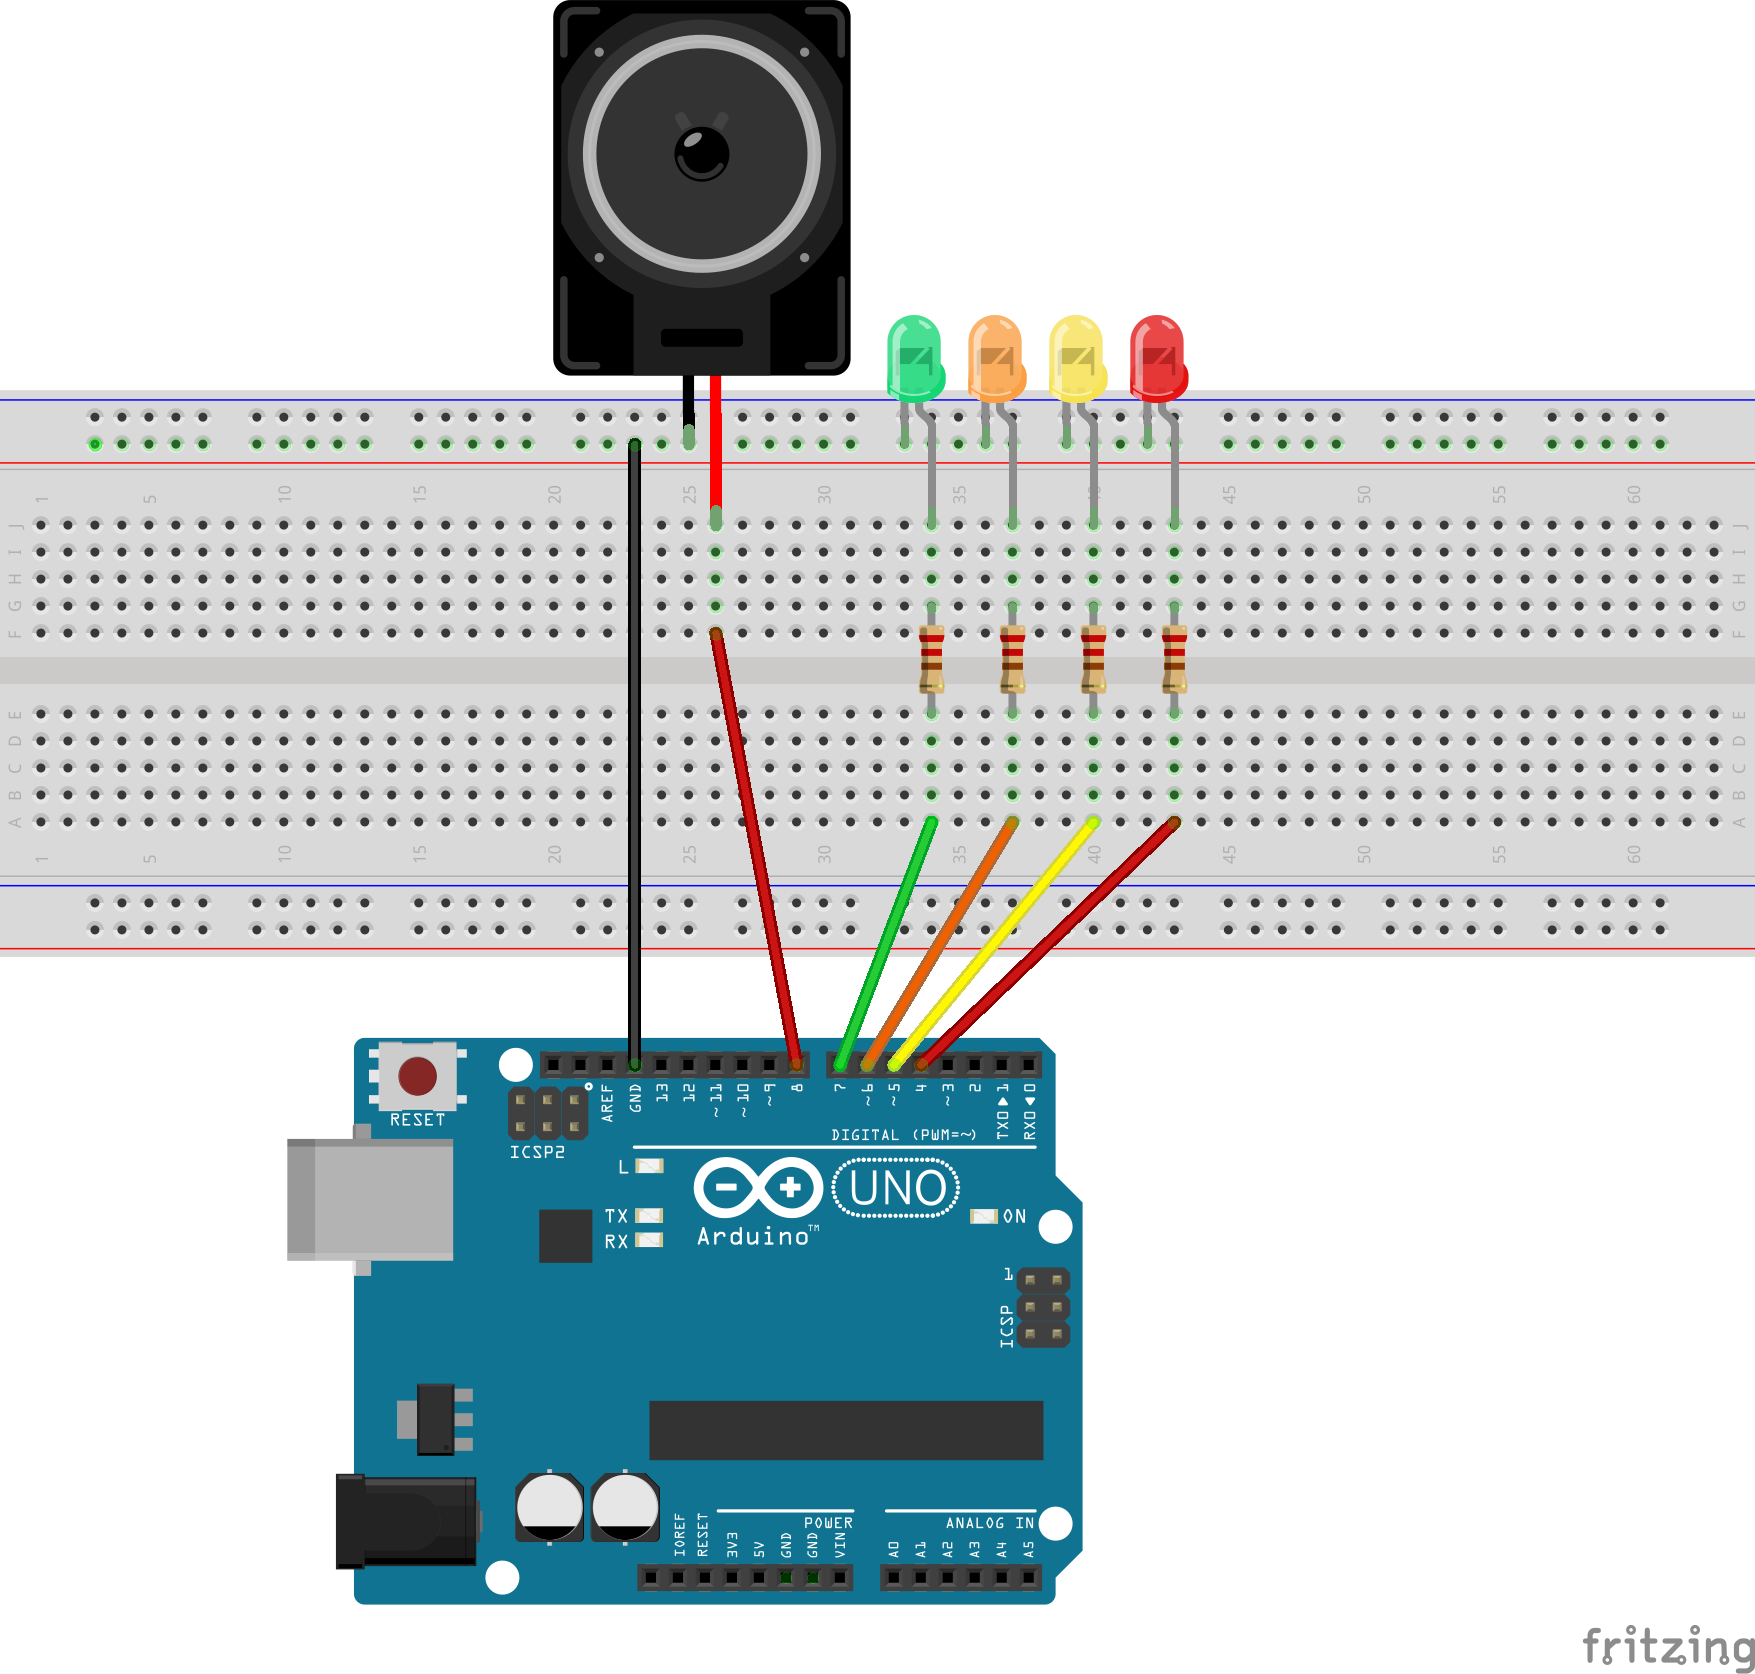
\includegraphics[scale=0.9]{images/schema_tests.png}
					\caption{Sch\'ema du prototype de test}
				\end{center}
			\end{figure}
			\begin{figure}
				\begin{center}
					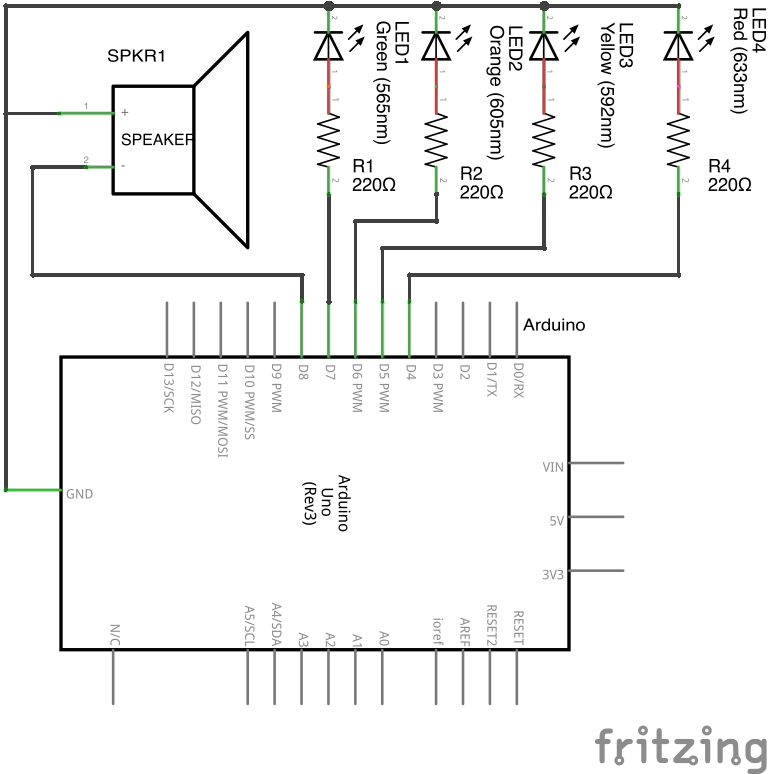
\includegraphics[scale=1]{images/schema_tests_elec.png}
					\caption{Sch\'ema \'electrique du prototype de test}
				\end{center}
			\end{figure}
		\section{Tests finaux}
			%TODO
		\section{Discussion et analyse}
	\chapter*{Conclusion}
\appendix
	\chapter{Code des applications}
		%Modifications de l'affichage des codes source
		\lstset{
			numbers = left,
			showspaces = none,
			keepspaces = true,
			showstringspaces = true,
			basicstyle = \footnotesize,
			commentstyle = \color{newGreen},
			keywordstyle = \color{newOrange},
			identifierstyle = \color{newBlue},
			stringstyle = \color{newMauve}
		}
		\lstdefinestyle{arduino}{
			language=C,
			morekeywords = {HIGH, LOW, INPUT, OUTPUT}
		}
		\section{Application principale}
			\lstinputlisting[language=python]{../Application_finale/app.py}
		\section{Code Arduino pour les tests}
			\lstinputlisting[style=arduino]{../src/tests/tests.ino}
	%TODO~: bibliographie
\end{document}